\subsubsection{Description}

All the cells that can be instantiated are listed below.\\
\indent These cells are generators which are proportionned thanks to parameters.
    
\subsubsection{List}

\begin{itemize}
    \item \verb-And2-  : \verb-q <= i0 & i1-
    \item \verb-And3-  : \verb-q <= i0 & i1 & i2-
    \item \verb-And4-  : \verb-q <= i0 & i1 & i2 & i3-
    \item \verb-Nand2- : \verb-nq <= ~ ( i0 & i1 )-
    \item \verb-Nand3- : \verb-nq <= ~ ( i0 & i1 & i2 )-
    \item \verb-Nand4- : \verb-nq <= ~ ( i0 & i1 & i2 & i3 )-
    \item \verb-Or2-   : \verb-q <= i0 & i1-
    \item \verb-Or3-   : \verb-q <= i0 & i1 & i2-
    \item \verb-Or4-   : \verb-q <= i0 & i1 & i2 & i3-
    \item \verb-Nor2-  : \verb-nq <= ~ ( i0 & i1 )-
    \item \verb-Nor3-  : \verb-nq <= ~ ( i0 & i1 & i2 )-
    \item \verb-Nor4-  : \verb-nq <= ~ ( i0 & i1 & i2 & i3 )-
    \item \verb-Inv-   : \verb-nq <= ~ i-
    \item \verb-Buf-   : \verb-q <= i-
    \item \verb-Xor2-  : \verb-q <= i0 ^ i1-
    \item \verb-Nxor2- : \verb-nq <= ~ ( i0 ^ i1 )-
    \item \verb-Zero-  : \verb-nq <= '0'-
    \item \verb-One-   : \verb-q <= '1'-
    \item \verb-Halfadder- : \verb-sout <= a ^ b- and \verb-cout <= a & b-
    \item \verb-Fulladder- : \verb-sout <= a ^ b ^ cin-\\\indent and \verb-cout <= ( a & b ) | ( a & cin ) | ( b & cin )-
    \item \verb-Sff- : \verb-if RISE ( ck ) : q <= i-
\end{itemize}

\subsubsection{Parameters}

The parameter \verb-'nbit'- gives the size of the generator. It is given through the dictionnary named \verb-param- (the default value is 1).

\subsubsection{Mapping file}

In order to map the virtual library, on has to write a .xml file which makes correspond models and interfaces. Note that the interfaces of the cells must be the same (except for the names of the ports). Otherwise, one has to create .vst files in order to make the interfaces match.\\
\indent By default, the mapping is done with sxlib library. There is an example of the .xml file below.\\
\indent The environment variable used to point the right file is \verb-STRATUS_MAPPING_NAME-.
\begin{figure}[hbp]
\centering
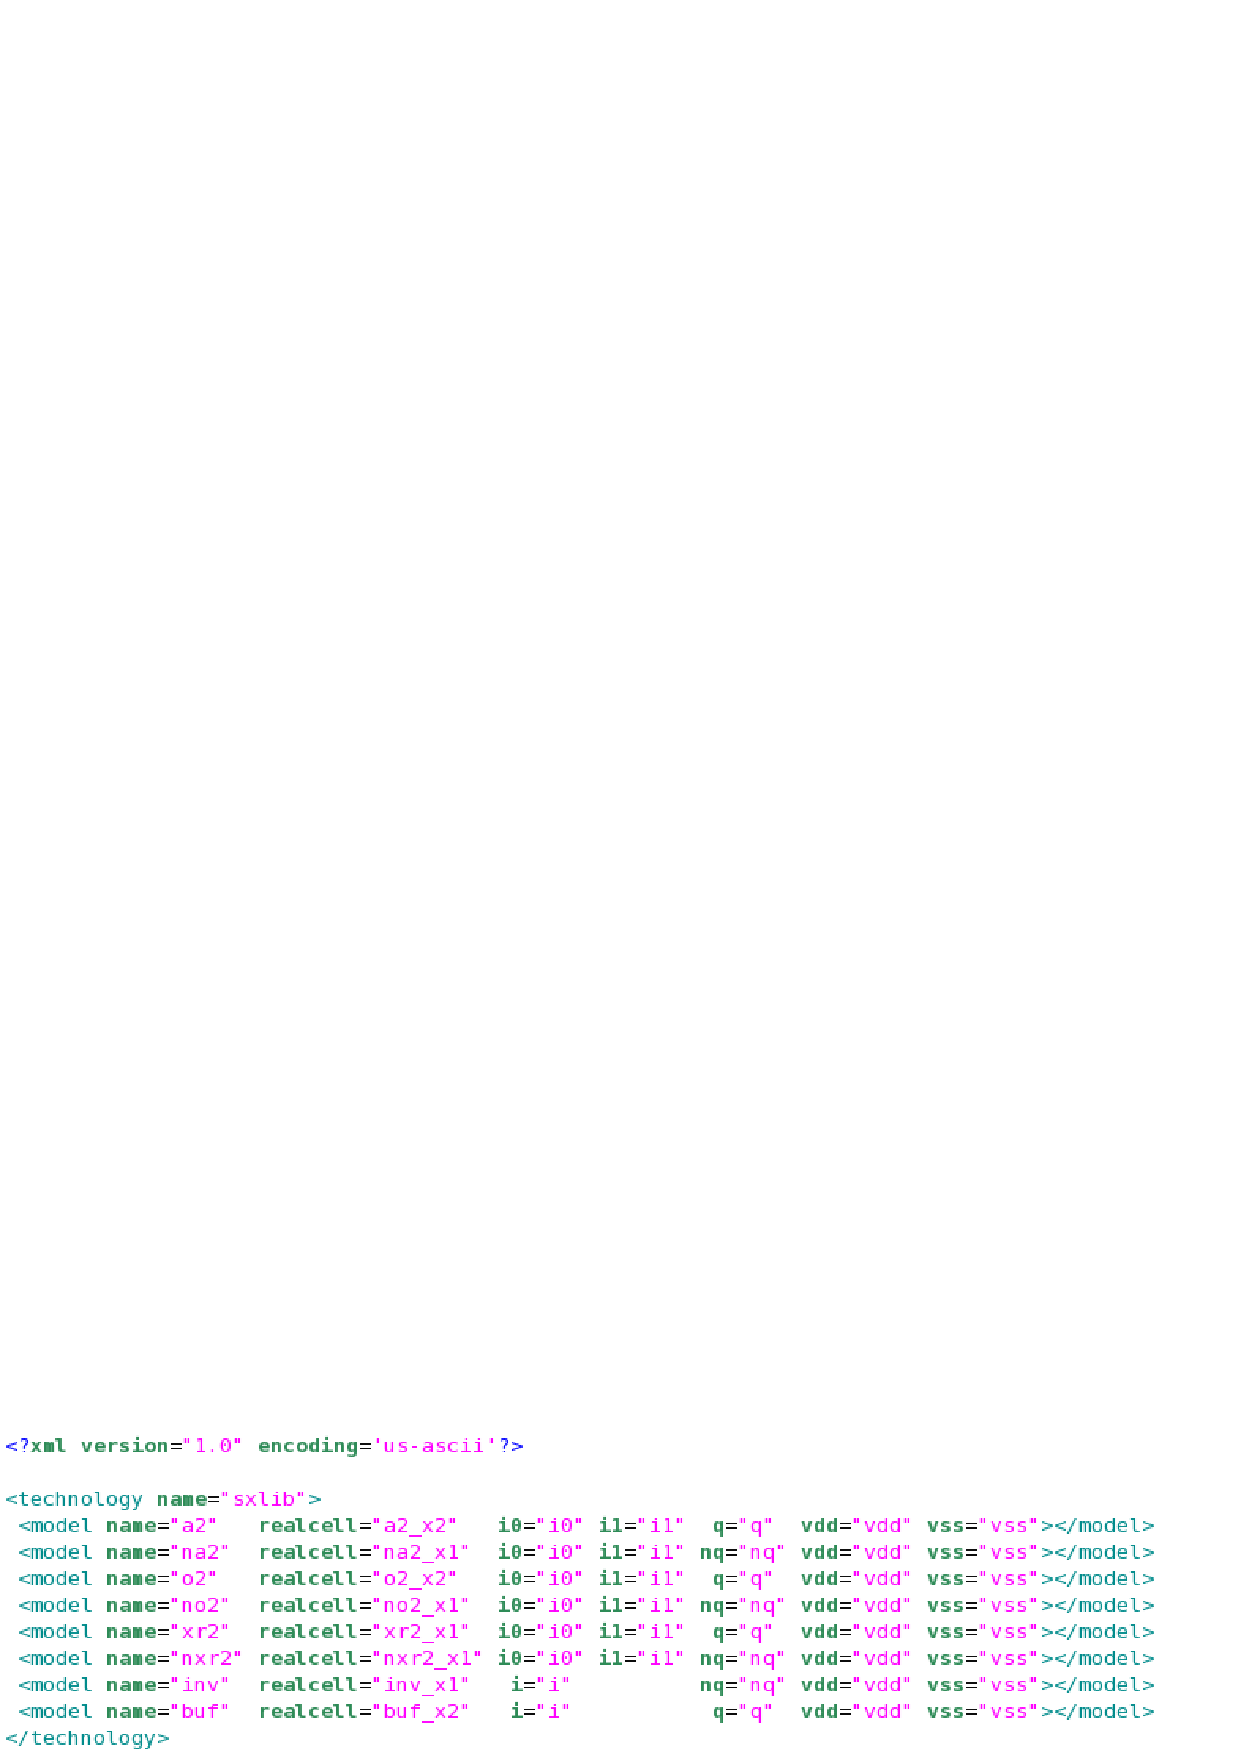
\includegraphics[width=1.3\textwidth]{images/xml.png}
\end{figure}

\subsubsection{Example}

\begin{verbatim}
Inst ( 'And2'
     , param = { 'nbit' : 4 }
     , map  = { 'i0'  : A
              , 'i1'  : B
              , 'q'   : S
              , 'vdd' : vdd
              , 'vss' : vss
              }
     )
\end{verbatim}

\subsubsection{Errors}
    
Some errors may occur :
\begin{itemize}
    \item \verb-[Stratus ERROR] Inst : the model ... does not exist.-\\\verb-Check CRL_CATA_LIB.-\\The model of the cell has not been found. One has to check the environment variable.
    \item \verb-[Stratus ERROR] Virtual library : No file found in order to parse.-\\\verb-Check STRATUS_MAPPING_NAME.-\\The mapping faile is not given in the environment variable.
\end{itemize} 

\subsubsection{See Also}

\hyperref[ref]{\emph{Introduction}}{}{Introduction}{secintroduction}

